%%%%%%%%%%%%%%%%%%%%%%% CHAPTER - 3 %%%%%%%%%%%%%%%%%%%%\\
\chapter{Intrusion Detection System}
\label{C3} %%%%%%%%%%%%%%%%%%%%%%%%%%%%
\graphicspath{{Figures/PDF/}{Figures/PNG/}}

\noindent\rule{\linewidth}{2pt}
\noindent
The computer systems and the networks of these systems are increasing day by day and security of data share by these networks is being an issue over the years. Security techniques of classical networks cannot be applied here because WSN has certain limitations of resources like energy, memory, CPU etc. Security mechanism of network must be able to ensure Confidentiality, Integrity, Availability and Authenticity.
\section{Intrusion and Intrusion Detection}
An intrusion in any system is an attempt to unauthorized access of system's data or resources. This unauthorized access can be limited to only monitoring and analyzing traffic patterns or it can be an attempt to modify or alter the data packets. Try to make resources busy and unavailable for the intended authorized access is also an intrusion attack. An intrusion detection system basically monitors and analyzes the network traffic for any suspicious activity by any of the network node. IDS tries to analyze network behavior and monitors user activity. IDS comes under passive defence category as these system tries to detect intrusion attack rather than preventing attack. These systems can only capable of reporting and alarming to administration to take some action. An IDS which can also take some required action to prevent the attack on its own, is known is Intrusion prevention System (IPS). An ideal IDS tries to minimize false positive rate with high detection rate. Also less energy consumption and faster computation or attack detection is desired feature of IDS. Main components of any IDS is shown in figure \ref{IDS-Component} \cite{alrajeh2013intrusion} are -
\begin{enumerate}[label=\textbf{\roman*}]
\item \textbf{Monitoring} This component mainly monitors traffic in the network, availability of resources. Events at each node, network congestion, packet delay, neighbor monitoring is also done by monitoring component.
\item \textbf{Analysis and Detection} This module of IDS implements the detection method for intrusion. It is the main component in the IDS where all monitored traffic patterns, events are analyzed to make decision regarding maliciousness of a node.
\item \textbf{Alarm} Alarm component is responsible for generating responses as alarm to administration if a malicious activity is detected.
\end{enumerate}
\begin{figure}[tp]
\center	
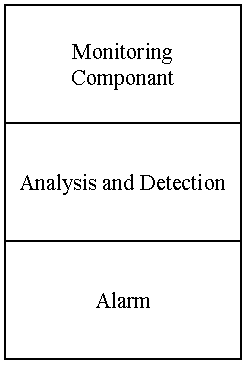
\includegraphics[width=1.75in, height=2.5in] {Figures/PDF/IDS-Components.pdf}
\caption{Components of IDS}
\label{IDS-Component}	
\end{figure}
\par
\section{IDS vs IPS}
An IDS is a tool which either installed at network strategic points or at each host to detect any suspicious or malicious behavior. If any such behavior is found which can harm the system nodes or system's activity it notifies to the concerned authority. An IPS can perform all tasks of IDS, in addition to that it can also take desired action on its own to prevent the attack.
\section{Classification of IDS}
IDS classification has two broad categories - Signature-based and Anomaly-based, which are based on intrusion detection strategy. IDS can also be classified based on the location of data in two categories - Host-based and Network-based. More classification categories are shown in figure \ref{IDS-Classification} \cite{alrajeh2013intrusion, farooqi2009intrusion} are described below.

\begin{figure}[ht]
\center	
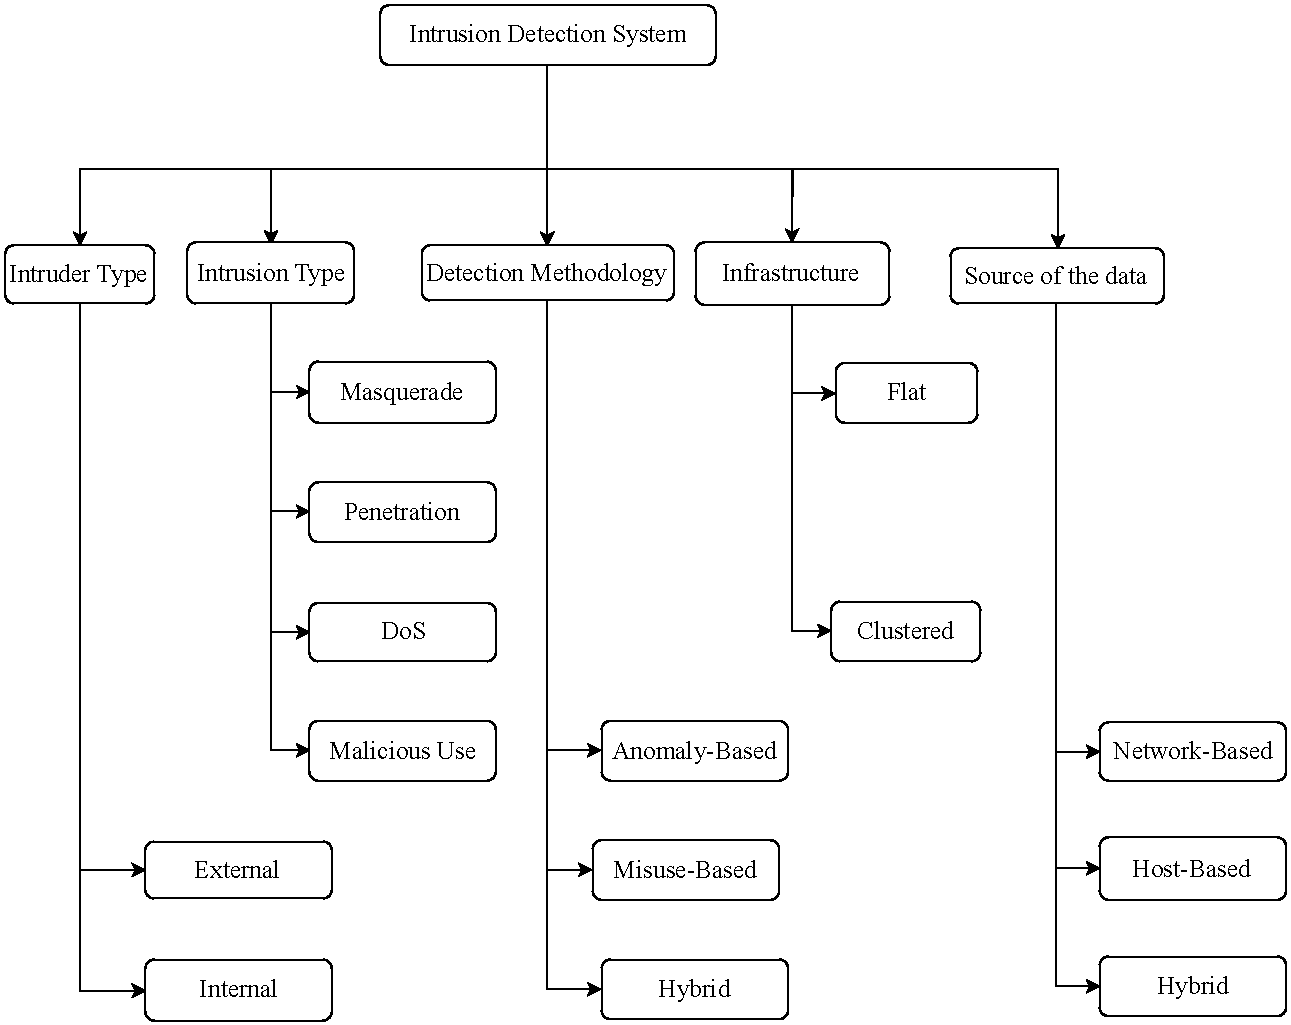
\includegraphics[width=\textwidth, height=5in] {Figures/PDF/IDS_Classification.pdf}
\caption{Classification of IDS}
\label{IDS-Classification}	
\end{figure}

\subsection{Detection Method}
IDS functionality is defined by the detection method. It describes how a detection system will behave in order to detect any malicious activity in the network. Research field in WSN mainly focuses on these following detection methods.
\begin{description}
  \item[$\bullet$ Anomaly-based] Anomaly-based IDS uses heuristic approaches to classify network activities as malicious or normal. This detection method finds the deviation from normal behavior and uses threshold value to classify attacks. To flag operation as an anomaly, the regular observation of system must be there to accommodate system changes. This may lead to performance overhead. This type of system can detect previously unknown attacks and sometimes fail to detect well-known attack. In [4] an IDS is proposed which is capable of learning and detecting new attacks using unsupervised neural network. Anomaly-based detection can be Statistical based, Knowledge-based or Machine learning based.
  \item[$\bullet$ Misuse-based (Signature or Rule-based)] In this detection method we have predefined rules against attacks to tackle them. Using this method one can detect previously known attack with high detection rate by comparing the new attack signature with known signatures and predefined rules. If there is a new attack, signature-based detection would not be able to compare with any reference signature (profile) hence this attack won’t be detected. In \cite{ioannis2007towards, krontiris2007intrusion}, a signature based IDS is presented. Every node has IDS so it is host based IDS. The architecture design for \cite{ioannis2007towards} is such that it detects data-packet drop and false routing attack and \cite{krontiris2007intrusion} is designed to detect only sinkhole attack.
  \item[$\bullet$ Hybrid IDS] These systems uses the combination of Anomaly-based and Misuse-based detection to detect new attacks using learning algorithms and  to detect well-known attacks, respectively. Hybrid systems are more efficient in terms of detection rate with low false positive rate. Also, these system uses high computation and hence results in more energy consumption. A hybrid IDS is proposed in \cite{li2008intruder} which uses distributive algorithm to train support vector machine (SVM) and create misuse detection model.
\end{description}
\subsection{Source of data}
IDS can be classified in 3 categories based upon the location of the data. It describes the location of the data where it is monitored. Data can be monitored on individual nodes or on the strategic point of network.
\begin{description}
    \item[$\bullet$ Network-Based] NIDS are deployed at strategic points so that it can monitor the packets transmission in network that is coming and going out to all network devices. This monitoring of data is then analyzed and compared with the signatures of known attacks. It is easy to deploy on the network boundary  with low cost where it can monitor all traffic.
    \item[$\bullet$ Host-Based] HIDS is implemented on individual host systems in the network and monitors all incoming and outgoing traffic instead of the whole network. HIDS is more helpful if the malicious node is inside the network.
    \item[$\bullet$ Hybrid IDS] It uses mobile agents to efficiently use a combination of NIDS and HIDS. Performance of hybrid IDS of better in terms of detection rate compared to NIDS and HIDS but hybrid system consumes more energy in detection process.
\end{description}
\subsection{Intruder Type}
IDS classification based on  an intruder node can be of two types - internal and external. It describe the location of the compromised node. In External intruder, attacker or compromised node is not present in the network whereas in case of internal intruder, it is present in the network. Internal intruder further can be classified as selfish node and malicious node in the way in which they affect the network's operation. Selfish node uses the network to forward own data packets, saves battery life for own operations, no cooperation in data forwarding, no direct damage to other nodes. On the other hand, malicious node damages other nodes, not focused on saving own battery life, tries to damage network services.
\subsection{Intrusion Type}
It describes a way of attack in which system is compromised. In Masquerade attack, attacker uses fake identity to gain unauthorized access. Penetration is an attempt to unauthorized access by breaching networks security. In DoS attack, attacker node tries to extra use of network resource so authenticated users can’t access resources. Malicious Use of resources is an attack on network resource.

\subsection{Infrastructure Type}
IDS can be classified into 2 groups based on network infrastructure - Flat and Clustered. In flat infrastructure, all nodes can participate in all networking activities because it is assumed that all the nodes in the network have equal capabilities. In Clustered, nodes are grouped which is known as clusters and each group is assigned a head known as cluster head.

%%%%%%%%%%%%%%%%%%%%%%%%%%%%%%%%%%%%%%%%%%%%%%%%%%%%%%%%%%%%%%%%%%%%%%%%%%%%%%%%%%%%%%%%%%%%%%%%%%%%%%%%%%%%%%%%%%%%%%%%%%%%%%%%%%%%%%%

%%%%%%%%%%%%%%%%%%%%%%%%%%%%%%%%%%%%%%%%%%%%%%%%%%%%%%%%%%%%%%%%%%%%%%%%%%%%%%%%%%%%%%%%%%%%%%%%%%%%%%%%%%%%%%%%%%%%%%%%%%%%%%%%%%%%%%%

%%%%%%%%%%%%%%%%%%%%%%%%%%%%%%%%%%%%%%%%%%%%%%%%%%%%%%%%%%%%%%%%%%%%%%%%%%%%%%%%%%%%%%%%%%%%%%%%%%%%%%%%%%%%%%%%%%%%%%%%%%%%%%%%%%%%%%%